\documentclass[12pt,hyperref,a4paper,UTF8]{ctexart}
\usepackage{CUGReport}
\usepackage{listings}
\usepackage{xcolor}
\usepackage{fontspec}
\usepackage{setspace}
\setstretch{1.5} % 设置全局行距为1.5倍
\usepackage[linesnumbered,ruled,vlined]{algorithm2e}
\usepackage{enumitem}
\setlist[itemize]{itemsep=0pt, parsep=0pt}
\usepackage{amsmath}
\usepackage{amsfonts}
\usepackage{amssymb}
\usepackage{graphicx}
\usepackage{booktabs}
\usepackage{caption}
\usepackage{subfigure}
% \usepackage{subcaption}
\usepackage{longtable}
\usepackage{float}
\usepackage{hyperref}
\usepackage{natbib}

% 全文字体:中文宋体,英文和数字 Times New Roman
\setCJKmainfont{SimSun}
\setmainfont{Times New Roman}

% 字号命令
\newcommand{\xiaochuhao}{\fontsize{36pt}{\baselineskip}\selectfont}
\newcommand{\erhao}{\fontsize{21pt}{\baselineskip}\selectfont}
\newcommand{\xiaoerhao}{\fontsize{18pt}{\baselineskip}\selectfont}
\newcommand{\sanhao}{\fontsize{15.75pt}{\baselineskip}\selectfont}
\newcommand{\sihao}{\fontsize{14pt}{18pt}\selectfont}
\newcommand{\xiaosihao}{\fontsize{12pt}{18pt}\selectfont}

% 封面
{
	\title{
		\vspace{1cm}
		\songti \erhao \textbf{钻柱系统粘滑振动非线性机理分析\\与主动抑制策略研究} \par
		\vspace{1cm}
		\songti \sihao {\textbf{曾康慧}} \par
		\vspace{13cm}
	}
}

%%------------------------document环境开始------------------------%%
\begin{document}
	
	%%-----------------------封面--------------------%%
	\cover
	\thispagestyle{empty}
	
	%%------------------摘要-------------%%
	\newpage
	\begin{abstract}

随着石油天然气勘探向深井、超深井领域拓展,钻柱系统的振动问题日益突出。其中,扭转形式的粘滑振动(Stick-Slip Vibration)是危害最大的一种自激振动形式,严重影响钻进效率与设备安全。本文针对深井钻柱系统的粘滑振动问题,开展了动力学建模、机理分析及主动控制策略研究。首先,基于集总参数法建立了包含转盘、钻杆、底部钻具组合(Bottom Hole Assembly, BHA)及钻头的四自由度非线性扭转动力学模型,重点引入了基于Stribeck效应的钻头-岩石非线性摩擦模型。其次,通过MATLAB/Simulink仿真深入分析了粘滑振动的产生机理,探讨了钻压、转速等工程参数对振动特性的影响,并对比了不同常微分方程(ODE)求解器在刚性系统求解中的精度与效率。最后,为有效抑制粘滑振动,设计了基于极点配置的状态观测器反馈控制策略,并与常规PID(Proportional-Integral-Derivative)控制进行了对比验证。仿真结果表明,所提出的观测器反馈控制策略能够更快速、有效地消除粘滑振动,实现钻头转速对地面设定值的精确跟踪,具有较强的鲁棒性和工程应用价值。
		
		\textbf{关键词:} 粘滑振动;扰动抑制;PID控制;状态观测器反馈控制;钻柱系统
	\end{abstract}
	
	\thispagestyle{empty}
	
	%%--------------------------目录页------------------------%%
	\newpage
	\tableofcontents
	\thispagestyle{empty}
	
	%%------------------------正文页从这里开始-------------------%%
	\newpage
	\setcounter{page}{1}
	


%----------------------------------------------------------------------------------------
%	第一章 引言
%----------------------------------------------------------------------------------------
\section{引言}

\subsection{研究背景与意义}
能源是现代社会经济发展的命脉。随着全球浅层油气资源的日益枯竭,油气勘探开发的重点正逐步转向深层、超深层以及复杂地质环境。在深井钻探过程中,钻柱系统作为连接地面与井底的关键纽带,其长细比极大(数千米长的钻柱直径仅为十几厘米),在狭窄的井眼中极易受到极其复杂的载荷作用,导致系统发生剧烈的非线性动力学行为。

钻柱的振动形式主要包括轴向振动(Axial Vibration)、横向振动(Lateral Vibration)和扭转振动(Torsional Vibration)。其中,扭转振动常常演化为一种被称为“粘滑振动”的严重失稳现象。粘滑振动的特征表现为钻头转速在零(粘滞阶段)和数倍于地面转盘转速(滑脱阶段)之间剧烈波动\cite{Jansen1995}。这种剧烈的交变应力会导致钻具螺纹疲劳失效、钻头切削齿崩断、随钻测量仪器(MWD)损坏,进而造成钻井周期延长、成本增加甚至灾难性的井下事故\cite{Tucker2003}。因此,深入研究钻柱粘滑振动的产生机理,并探索高效的主动控制抑制策略,对于保障国家能源安全、提升复杂油气藏的勘探开发效率具有重要的理论意义和工程价值。

\subsection{国内外研究现状}
学术界和工业界对钻柱粘滑振动的研究由来已久。早期的研究主要集中在现象描述和机理分析上。Kyllingstad等\cite{Kyllingstad2019}指出,钻头与岩石相互作用中的非线性摩擦特性(即静摩擦力远大于动摩擦力)是导致粘滑振动的根本原因。随后,基于集总参数模型(Lumped Parameter Model)和有限元方法(FEM)的动力学建模成为主流\cite{Patil2018}。

在控制策略方面,被动控制主要通过优化钻具组合或调整钻井参数(如降低钻压、提高转速)来缓解振动,但往往以牺牲机械钻速(ROP)为代价。主动控制技术则通过调节顶部驱动系统的输出扭矩或转速来抑制井下振动,成为近年来的研究热点。软扭矩旋转系统(Soft Torque Rotary System)是目前应用最广泛的商业化技术,但在大深度、高摩擦工况下效果受限\cite{Liu2024}。为此,学者们提出了多种先进控制算法,包括PID控制\cite{Wang2021}、滑模控制(Sliding Mode Control, SMC)\cite{Li2021}、线性二次型高斯控制(LQG)\cite{Saldivar2016}以及自抗扰控制(ADRC)\cite{Zhang2022}等。然而,由于井下状态难以实时测量,基于状态观测器的控制策略因其能够利用地面可测信号估计井下状态而备受关注\cite{Navarro2020, Cheng2018}。

\subsection{本文主要工作}
本文针对现有研究中模型简化过度或控制策略难以工程实现的问题,开展了以下工作:
1. 建立了包含转盘、钻杆、BHA及钻头的四自由度非线性扭转动力学模型,精细刻画了钻柱系统的弹性特征及非线性摩擦行为。
2. 详细分析了不同钻井参数下粘滑振动的演化规律,并对比了不同数值求解算法的适用性。
3. 设计了基于LQR极点配置的全维状态观测器,提出了一种基于观测器的状态反馈控制策略,并与经典PID控制进行了系统性的对比仿真实验。

%----------------------------------------------------------------------------------------
%	第二章 钻柱系统动力学建模
%----------------------------------------------------------------------------------------
\section{钻柱系统的动力学建模}

钻柱系统是一个具有无限维自由度的连续弹性体,但在研究其低频扭转振动特性时,采用离散化的集总参数模型既能保证计算精度,又能显著降低计算复杂度,便于控制器设计。

\subsection{系统结构简化与假设}
典型的旋转导向钻井系统如图\ref{fig:rig_system}所示,主要由井架、转盘、钻杆、底部钻具组合(BHA)和钻头组成。

\begin{figure}[htbp]
	\centering
	\includegraphics[width=0.6\linewidth]{fig/钻井系统的基本组成}
	\caption{钻井系统的基本组成示意图\cite{巩全成}}
	\label{fig:rig_system}
\end{figure}

为了构建适用于控制系统设计的数学模型,我们将钻柱系统简化为四个集总质量块:转盘(Rotary Table)、钻杆(Drill Pipe)、BHA和钻头(Bit),如图\ref{fig:simplified_model}所示。
建模过程基于以下假设:
1. 井眼为垂直井,忽略井眼曲率影响。
2. 仅考虑钻柱的扭转自由度,忽略轴向和横向振动的耦合效应。
3. 钻杆与井壁之间的摩擦视为线性粘性阻尼。
4. 钻井液的影响等效为附加质量和阻尼。

\begin{figure}[htbp]
	\centering
	\includegraphics[width=0.6\linewidth]{fig/钻柱系统简化模型}
	\caption{四自由度钻柱系统简化集总参数模型}
	\label{fig:simplified_model}
\end{figure}

\subsection{动力学方程推导}
根据牛顿第二定律和扭转振动原理,四自由度系统的运动微分方程可描述如下:

转盘部分:
\begin{equation}
	J_{rs}\ddot{\theta}_{rs} + C_{rs}\dot{\theta}_{rs} + K_{rd}(\theta_{rs} - \theta_{dp}) + C_{rd}(\dot{\theta}_{rs} - \dot{\theta}_{dp}) = T_m
\end{equation}

钻杆部分:
\begin{equation}
	J_{dp}\ddot{\theta}_{dp} - K_{rd}(\theta_{rs} - \theta_{dp}) - C_{rd}(\dot{\theta}_{rs} - \dot{\theta}_{dp}) + K_{db}(\theta_{dp} - \theta_{bh}) + C_{db}(\dot{\theta}_{dp} - \dot{\theta}_{bh}) = 0
\end{equation}

BHA部分:
\begin{equation}
	J_{bh}\ddot{\theta}_{bh} - K_{db}(\theta_{dp} - \theta_{bh}) - C_{db}(\dot{\theta}_{dp} - \dot{\theta}_{bh}) + K_{bb}(\theta_{bh} - \theta_{pb}) + C_{bb}(\dot{\theta}_{bh} - \dot{\theta}_{pb}) = 0
\end{equation}

钻头部分:
\begin{equation}
	J_{bb}\ddot{\theta}_{bb} - K_{bb}(\theta_{bh} - \theta_{pb}) - C_{bb}(\dot{\theta}_{bh} - \dot{\theta}_{pb}) + C_{pb}\dot{\theta}_{pb} = -T_b
\end{equation}

其中,$J_i$ ($i \in \{rs, dp, bh, bb\}$) 表示各部分的转动惯量;$\theta_i$ 和 $\dot{\theta}_i$ 分别表示角位移和角速度;$K_{xy}$ 和 $C_{xy}$ 表示各部件之间的等效扭转刚度和阻尼;$T_m$ 为顶部驱动扭矩;$T_b$ 为钻头与岩石之间的非线性摩擦力矩。

\subsection{非线性摩擦模型}
钻头与岩石的交互作用是引起粘滑振动的核心非线性源。本文采用包含Stribeck效应的干摩擦模型,该模型能够准确描述静摩擦与动摩擦之间的转换过程。其数学表达式为:

\begin{equation}
	T_b(\dot{\theta}_{pb}) = W_b R_b \mu_b(\dot{\theta}_{pb}) \cdot \text{sgn}(\dot{\theta}_{pb})
\end{equation}

其中,$W_b$ 为钻压(Weight on Bit),$R_b$ 为钻头半径。摩擦系数 $\mu_b$ 定义为:

\begin{equation}
	\mu_b(\dot{\theta}_{pb}) = \mu_{cb} + (\mu_{sb} - \mu_{cb})e^{-\gamma_b |\dot{\theta}_{pb}|}
\end{equation}

式中,$\mu_{sb}$ 为最大静摩擦系数,$\mu_{cb}$ 为库伦摩擦系数,$\gamma_b$ 为衰减因子,决定了从静摩擦向动摩擦过渡的速度。典型的钻头摩擦力矩特性曲线如图\ref{fig:torque_model}所示。

\begin{figure}[htbp]
	\centering
	\includegraphics[width=0.6\linewidth]{fig/钻头摩擦力矩}
	\caption{钻头-岩石非线性摩擦力矩特性曲线(Stribeck效应)}
	\label{fig:torque_model}
\end{figure}

为了解决零速附近的数值奇异问题,在仿真中引入Karnopp摩擦模型,设置一个极小的速度阈值 $\xi$。当 $|\dot{\theta}_{pb}| < \xi$ 且驱动力矩小于最大静摩擦力矩时,钻头处于粘滞状态(Stick),此时钻头速度强制为零;否则钻头进入滑脱状态(Slip)。

\subsection{状态空间方程}
为了便于控制器的设计,选取状态变量向量 $\bm{x} = [\dot{\theta}_{rs}, \theta_{rs}-\theta_{dp}, \dot{\theta}_{dp}, \theta_{dp}-\theta_{bh}, \dot{\theta}_{bh}, \theta_{bh}-\theta_{pb}, \dot{\theta}_{pb}]^T$。系统可转化为如下标准状态空间形式:

\begin{equation}
	\begin{cases}
		\dot{\bm{x}}(t) = \bm{A}\bm{x}(t) + \bm{B}u(t) + \bm{B}_d d(t) \\
		\bm{y}(t) = \bm{C}\bm{x}(t)
	\end{cases}
\end{equation}

其中,输入 $u(t) = T_m$,扰动 $d(t) = T_b$。由于井下数据传输带宽限制,通常只能实时测量地面转盘转速,因此输出方程中 $\bm{C}$ 矩阵仅对应转盘速度项。具体的系数矩阵 $\bm{A}, \bm{B}$ 详见附录中的推导。

%----------------------------------------------------------------------------------------
%	第三章 粘滑振动机理与开环仿真分析
%----------------------------------------------------------------------------------------
\section{粘滑振动机理与开环仿真分析}

\subsection{粘滑振动现象复现}
利用MATLAB/Simulink搭建上述非线性动力学模型。在未施加主动控制策略(即开环状态或仅有基础调速器)的情况下,设定目标转速为 12 rad/s,钻压为 97.347 kN。仿真结果如图\ref{fig:stick_slip_demo}所示。

\begin{figure}[htbp]
	\centering
	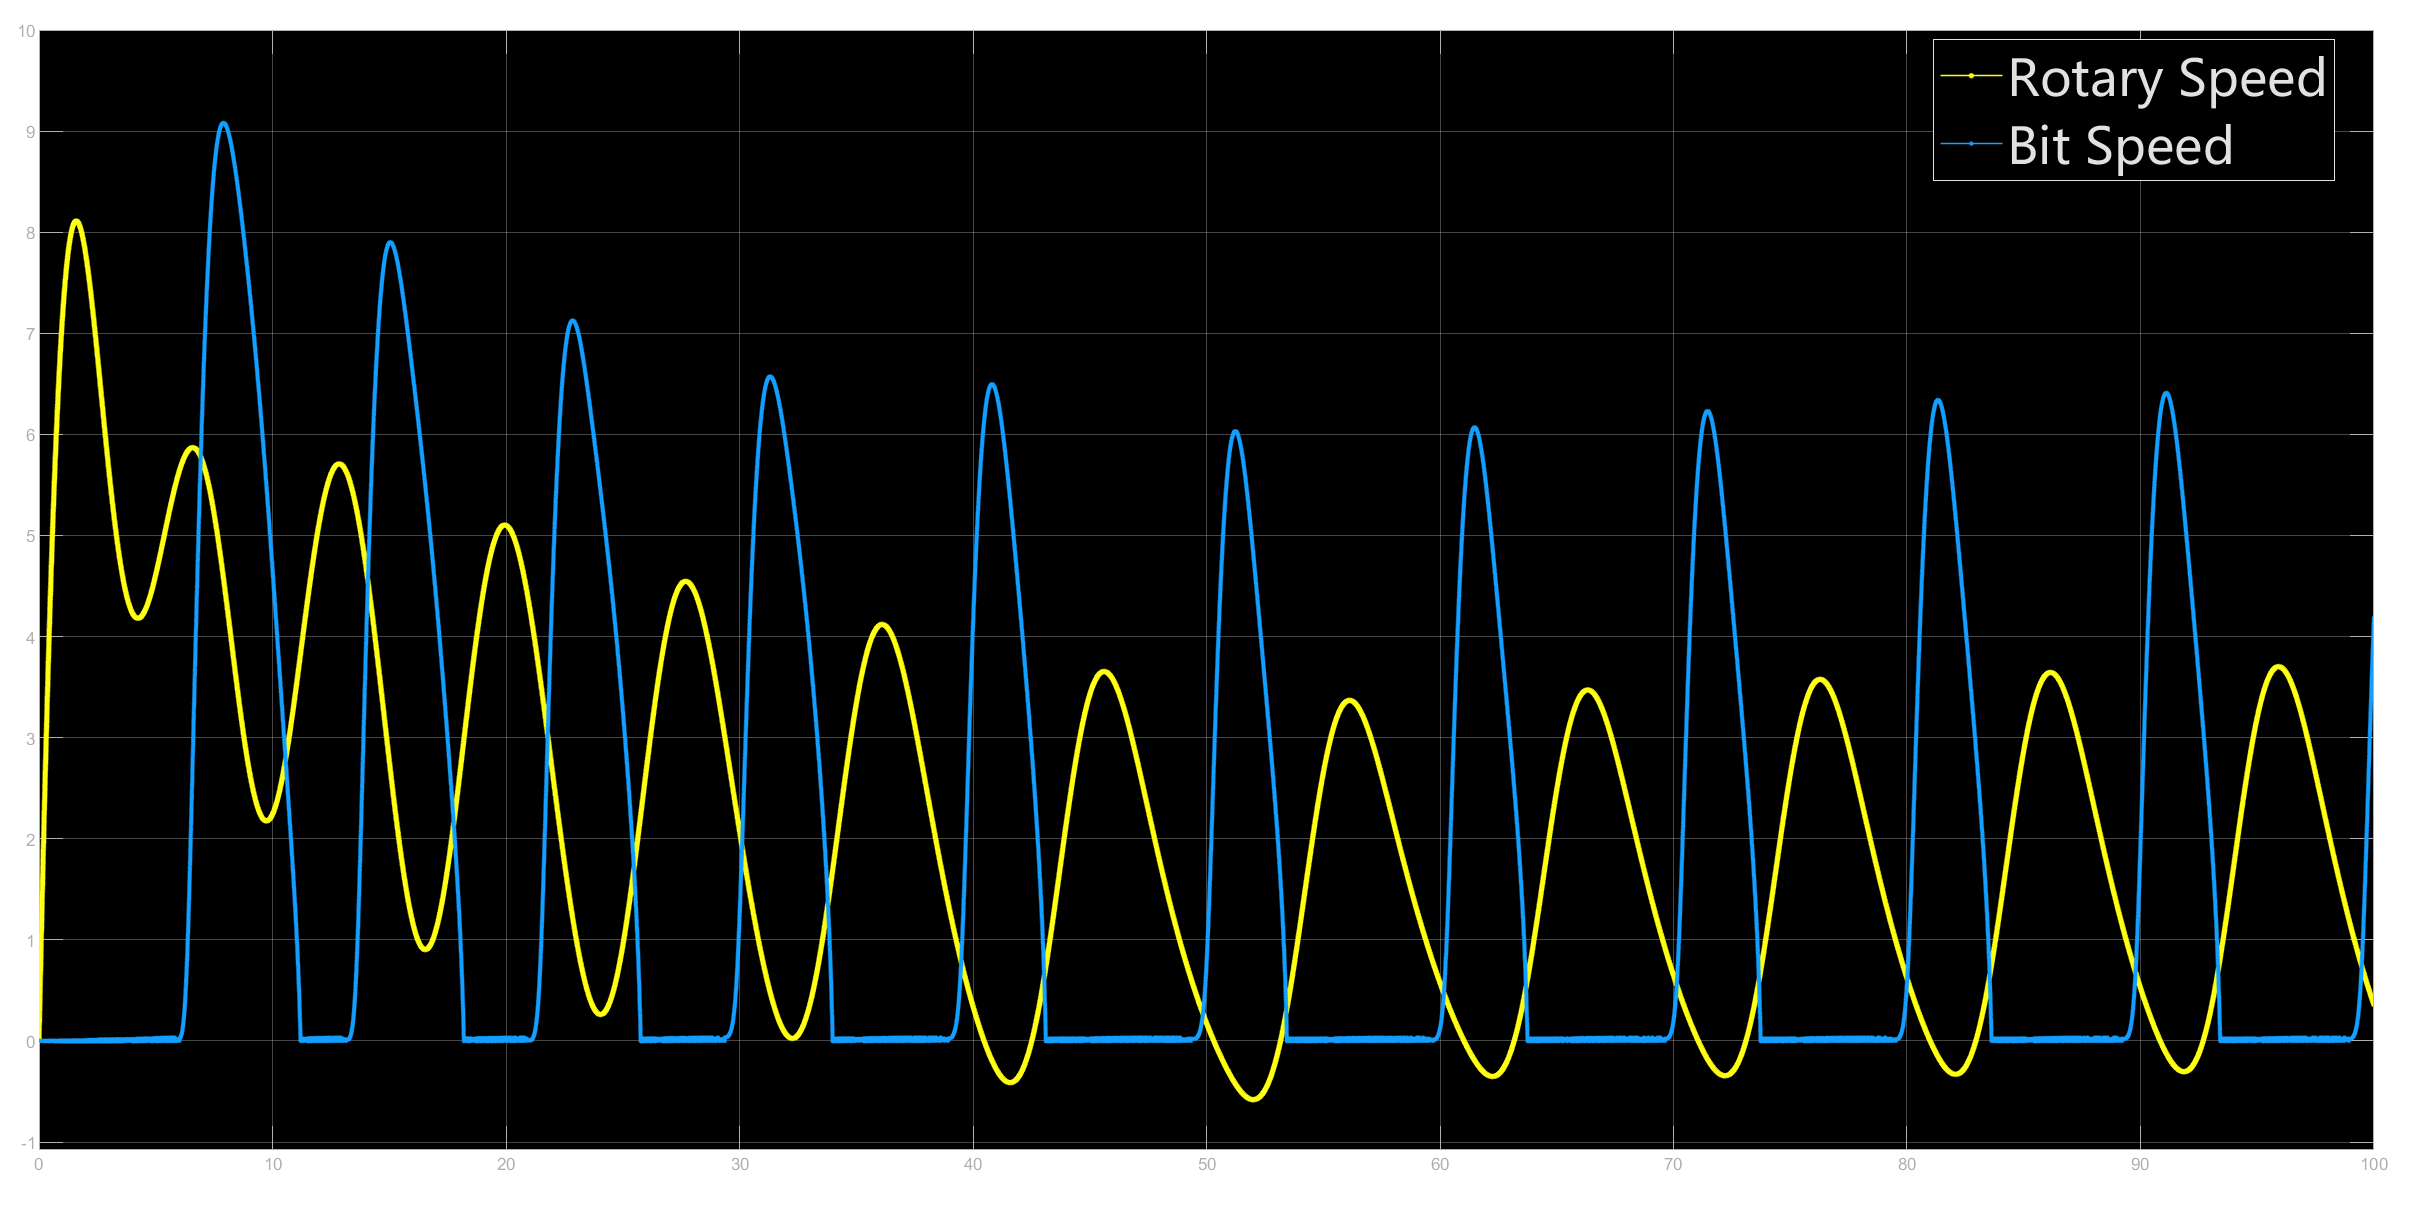
\includegraphics[width=0.8\linewidth]{fig/Rotary_Speed和Bit_Speed的粘滑振动}
	\caption{开环状态下的地面转速(蓝)与井下钻头转速(红)响应}
	\label{fig:stick_slip_demo}
\end{figure}

如图\ref{fig:stick_slip_示意}所示,钻头转速呈现出极其明显的周期性波动。在粘滞阶段,钻头转速为零,而地面转盘持续旋转,导致钻柱扭转能量急剧积聚;当累积扭矩突破静摩擦极限时,能量瞬间释放,钻头转速迅速飙升至地面转速的2-3倍(滑脱阶段),随后因动能耗散再次被“捕获”进入粘滞状态。这种极限环(Limit Cycle)行为正是粘滑振动的典型特征。

\begin{figure}[htbp]
	\centering
	\includegraphics[width=0.5\linewidth]{fig/钻柱粘滑振动示意图}
	\caption{粘滑振动过程中的钻柱扭转状态示意图}
	\label{fig:stick_slip_示意}
\end{figure}

\subsection{钻井参数敏感性分析}
钻压(WOB)是影响粘滑振动的关键参数之一。保持其他条件不变,分别测试了不同钻压下的系统响应。
如图\ref{fig:wob_effect1}所示,当钻压略微降低至90 kN时,虽然粘滞时间缩短,但振动依然存在。然而,如图\ref{fig:wob_effect2}所示,当钻压增加至107.2 kN时,巨大的静摩擦力矩导致钻头长时间陷入“死卡”(Lock-up)状态,甚至完全无法启动。这表明单纯依靠调整钻压难以在保证机械钻速的前提下消除粘滑振动。

\begin{figure}[htbp]
	\centering
	\subfigure[钻压减小工况]{
		\includegraphics[width=0.45\linewidth]{fig/W_b=90kN和W_b=85kN 时钻头角速度的变化}
		\label{fig:wob_effect1}
	}
	\subfigure[钻压增大工况]{
		\includegraphics[width=0.45\linewidth]{fig/W_b=98kN和W_b=107.2kN 时钻头角速度的变化}
		\label{fig:wob_effect2}
	}
	\caption{不同钻压条件下的钻头转速响应对比}
\end{figure}

\subsection{数值求解器的选择与精度分析}
钻柱系统由于包含非线性库伦摩擦及高频扭转模态,属于典型的刚性(Stiff)系统。为了确保仿真结果的可信度,本文对比了MATLAB中三种常用ODE求解器:`ode45`(显式Runge-Kutta)、`ode23`和`ode15s`(隐式求解器,专用于刚性问题)。

对比结果如图\ref{fig:ode_compare}所示。虽然三者在宏观趋势上一致,但在粘滞-滑脱转换的瞬态时刻,`ode45`提供了更平滑且符合物理规律的解,而低阶求解器在速度突变点存在较大的数值振荡。尽管`ode15s`在处理刚性方程时理论上更稳定,但在本模型的参数设置下,`ode45`在精度和计算时间上取得了最佳平衡。

\begin{figure}[htbp]
	\centering
	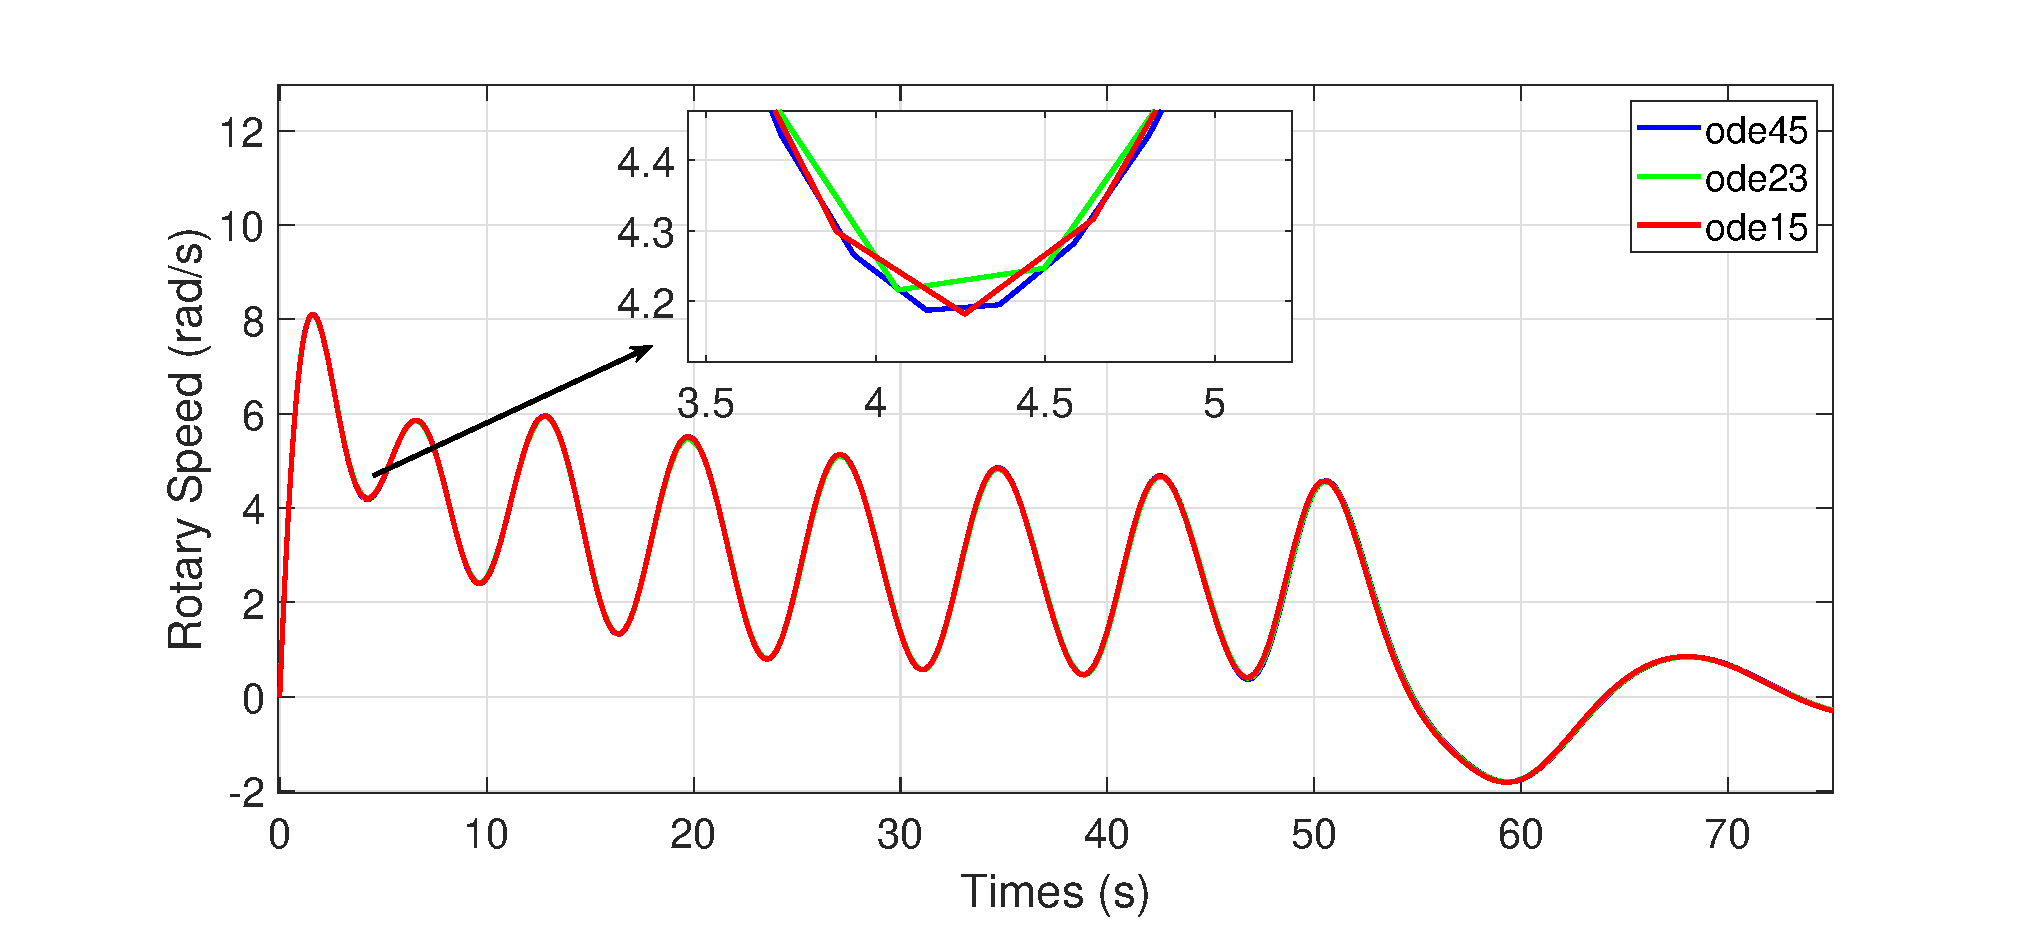
\includegraphics[width=0.7\linewidth]{fig/未加控制三种ode函数求解对比}
	\caption{不同ODE求解器在求解钻柱动力学方程时的结果对比}
	\label{fig:ode_compare}
\end{figure}

%----------------------------------------------------------------------------------------
%	第四章 主动抑制控制策略设计
%----------------------------------------------------------------------------------------
\section{主动抑制控制策略设计}

为了从根本上消除粘滑振动,需要引入主动反馈控制。本文提出了基于状态观测器的全状态反馈控制策略,并设计了PID控制器作为性能基准。系统整体控制架构如图\ref{fig:control_structure}所示。

\begin{figure}[htbp]
	\centering
	\includegraphics[width=0.8\linewidth]{fig/控制系统结构}
	\caption{基于观测器的钻柱系统主动控制架构框图}
	\label{fig:control_structure}
\end{figure}

\subsection{PID控制器设计}
PID控制是工业界最成熟的控制算法。针对钻柱系统,PID控制律设计为:
\begin{equation}
	u_{PID}(t) = K_p e(t) + K_i \int_{0}^{t} e(\tau)d\tau + K_d \frac{de(t)}{dt}
\end{equation}
其中,$e(t) = \Omega_{ref} - \dot{\theta}_{rs}$ 为转盘转速误差。如图\ref{fig:pid_model}所示,我们在Simulink中构建了PID控制回路。由于系统的大惯量特性,必须采用较大的比例增益$K_p$才能产生足够的矫正扭矩。

\begin{figure}[htbp]
	\centering
	\includegraphics[width=0.7\linewidth]{fig/PID控制模型}
	\caption{Simulink中的PID控制模型实现}
	\label{fig:pid_model}
\end{figure}

\subsection{状态观测器设计}
由于井下钻头转速 $\dot{\theta}_{pb}$ 无法实时测量,无法直接实现全状态反馈。因此,设计一个Luenberger状态观测器来重构不可测状态:
\begin{equation}
	\begin{cases}
		\dot{\hat{\bm{x}}} = \bm{A}\hat{\bm{x}} + \bm{B}u + \bm{L}(\bm{y} - \bm{C}\hat{\bm{x}}) \\
		\hat{\bm{y}} = \bm{C}\hat{\bm{x}}
	\end{cases}
\end{equation}
其中,$\hat{\bm{x}}$ 为状态估计向量,$\bm{L}$ 为观测器增益矩阵。增益 $\bm{L}$ 的选取需保证观测误差动态 $\dot{\bm{e}} = (\bm{A} - \bm{L}\bm{C})\bm{e}$ 的特征值位于复平面左半平面且其实部足够负,以确保估计收敛速度快于系统本身动态。本文采用极点配置法(Pole Placement)计算 $\bm{L}$ 矩阵。

\subsection{基于观测器的状态反馈控制}
结合内模原理(Internal Model Principle)以消除稳态误差,构建增广状态向量 $\bar{\bm{x}} = [\bm{x}^T, x_c]^T$。控制律设计为:
\begin{equation}
	u(t) = -\bm{K} \hat{\bar{\bm{x}}}(t) = -[\bm{K}_s \quad K_R] \begin{bmatrix} \hat{\bm{x}}(t) \\ x_c(t) \end{bmatrix}
\end{equation}
其中,$\bm{K}_s$ 为状态反馈增益,$K_R$ 为内模增益。反馈增益矩阵通过线性二次型调节器(LQR)理论优化得到,旨在最小化如下性能指标:
\begin{equation}
	J = \int_{0}^{\infty} (\bar{\bm{x}}^T \bm{Q} \bar{\bm{x}} + u^T R u) dt
\end{equation}
权重矩阵 $\bm{Q}$ 和 $R$ 的选取权衡了系统的响应速度与控制能量消耗。观测器子系统及其在Simulink中的实现分别如图\ref{fig:observer_sub}和\ref{fig:observer_sim}所示。

\begin{figure}[htbp]
	\centering
	\subfigure[观测器子系统内部结构]{
		\includegraphics[width=0.45\linewidth]{fig/状态观测器子系统}
		\label{fig:observer_sub}
	}
	\subfigure[观测器控制回路实现]{
		\includegraphics[width=0.45\linewidth]{fig/状态观测器控制}
		\label{fig:observer_sim}
	}
	\caption{状态观测器及其控制系统的Simulink实现}
\end{figure}

%----------------------------------------------------------------------------------------
%	第五章 仿真实验与结果分析
%----------------------------------------------------------------------------------------
\section{仿真实验与结果分析}

\subsection{观测器性能验证}
首先验证状态观测器的估计精度。设定系统初始状态为零,在 $t=0$ 时刻施加阶跃转速指令。如图\ref{fig:obs_performance}所示,观测器估计的钻头转速(红色虚线)能够极快地收敛并精确跟踪实际模型的钻头转速(蓝色实线)。即使在系统发生剧烈非线性振荡的阶段,观测误差也保持在极小范围内,证明了所设计的观测器具有优异的动态重构能力。

\begin{figure}[htbp]
	\centering
	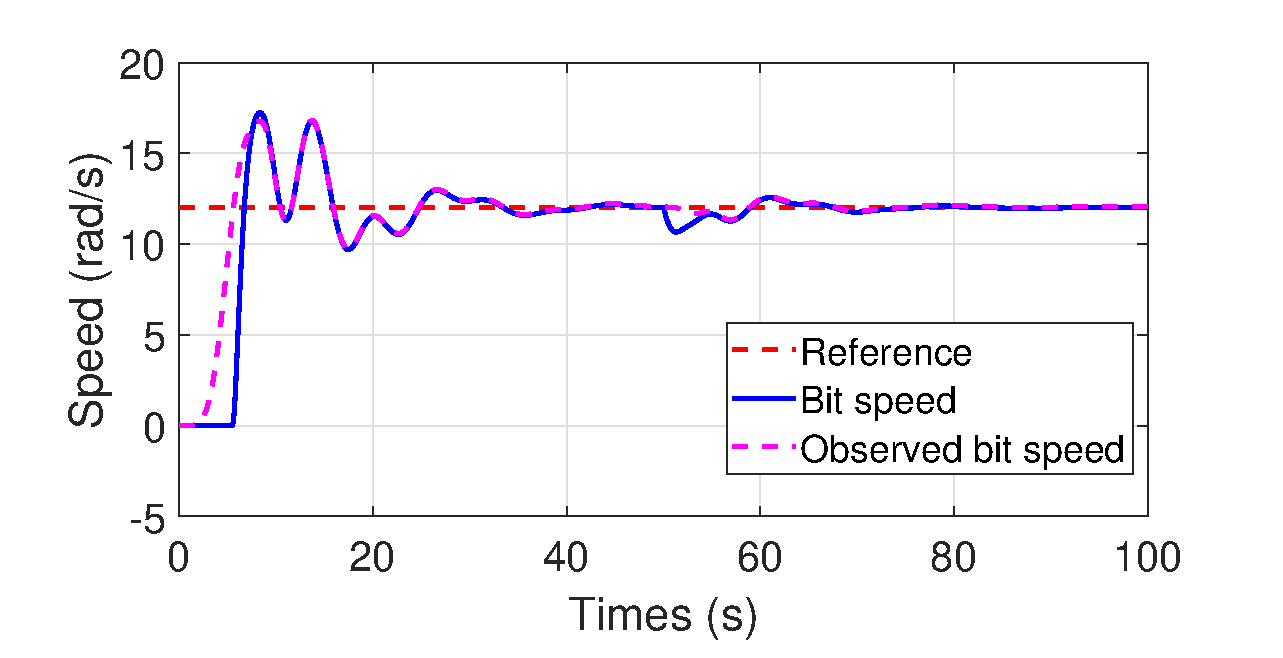
\includegraphics[width=0.7\linewidth]{fig/状态观测器观测效果}
	\caption{观测器对不可测状态(钻头转速)的估计效果验证}
	\label{fig:obs_performance}
\end{figure}

\subsection{控制策略对比分析}

\subsubsection{PID控制效果}
对PID控制器进行了多组参数整定。如图\ref{fig:pid_tuning}所示,随着比例增益 $P$ 和积分增益 $I$ 的增加,系统的响应速度加快,稳态误差减小。当 $P=1500, I=300$ 时,地面转速的波动得到了一定程度的抑制,但钻头转速(未展示)仍存在残余波动,且过高的增益可能导致控制扭矩饱和或引发高频噪声放大。

\begin{figure}[htbp]
	\centering
	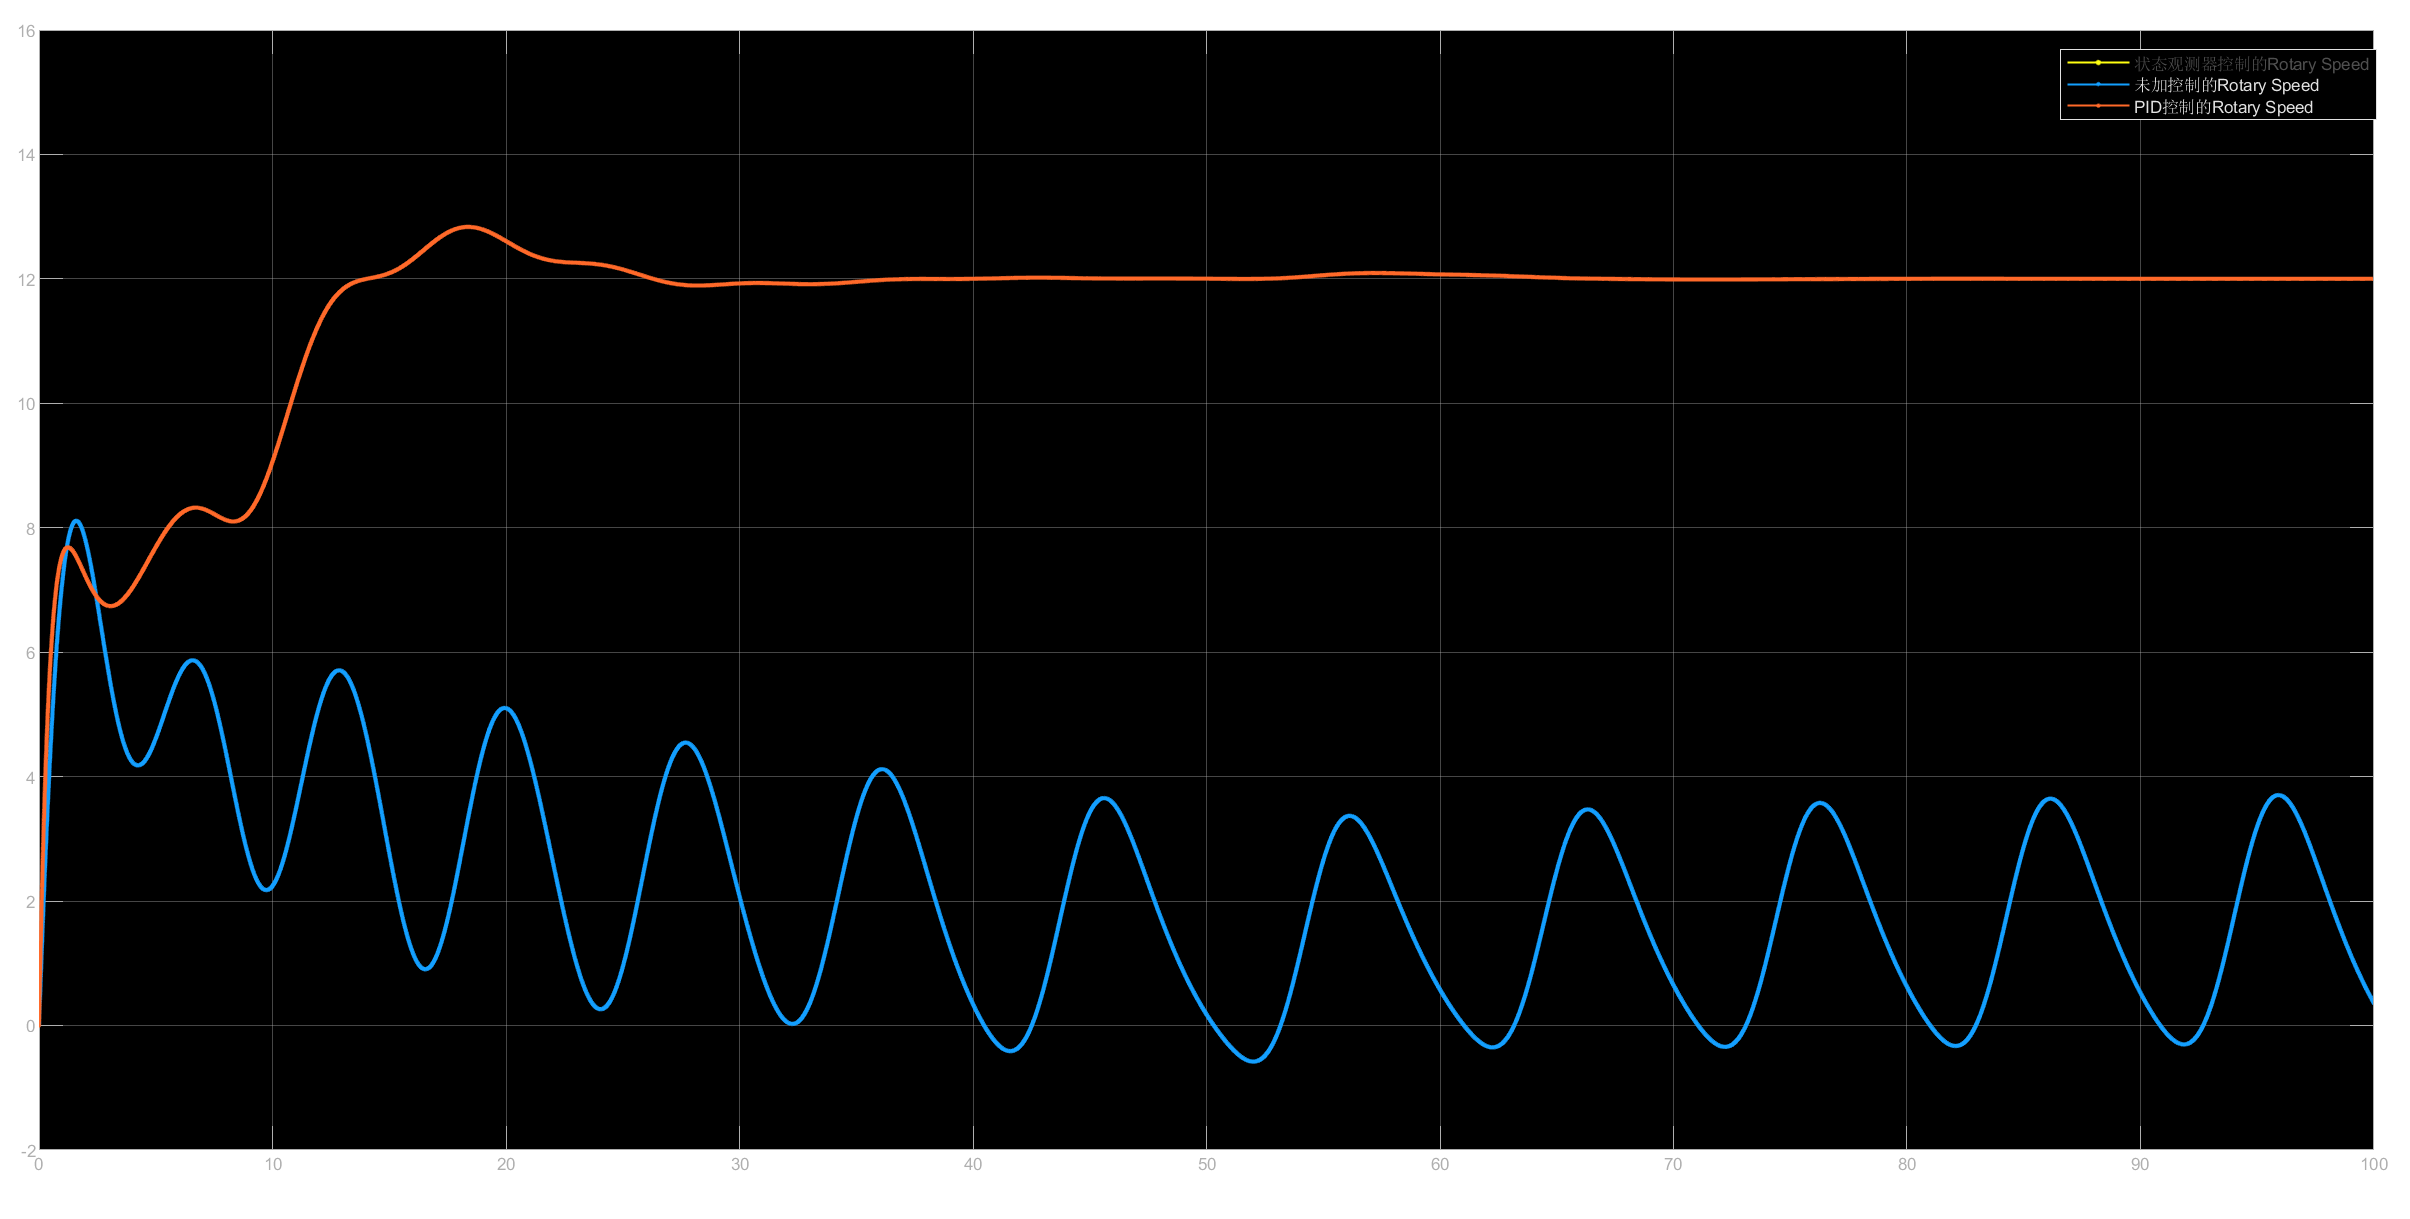
\includegraphics[width=0.7\linewidth]{fig/Rotary_Speed_PID控制_P1500_I300}
	\caption{优化参数后的PID控制下地面转速响应 ($P=1500, I=300$)}
	\label{fig:pid_tuning}
\end{figure}

\subsubsection{观测器反馈控制效果}
图\ref{fig:obs_control_result}展示了基于观测器的状态反馈控制效果。可以看出,该控制器能够迅速抑制系统的瞬态振荡。在约10秒内,钻头彻底摆脱了粘滑状态,转速平稳收敛至设定值 12 rad/s。与开环情况相比,系统不仅消除了极限环,还显著缩短了过渡过程时间。

\begin{figure}[htbp]
	\centering
	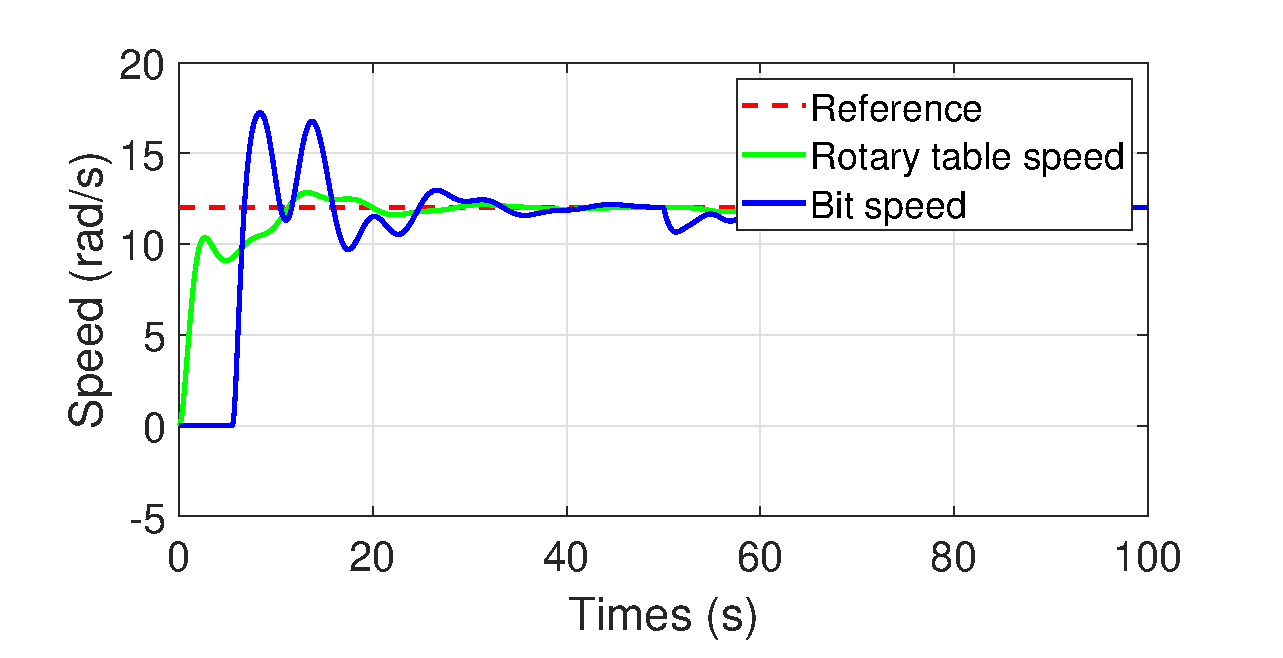
\includegraphics[width=0.7\linewidth]{fig/状态观测器控制效果}
	\caption{基于观测器的状态反馈控制下的系统响应(上:转盘,中:差速,下:钻头)}
	\label{fig:obs_control_result}
\end{figure}

\subsubsection{综合对比}
为了直观展示两种控制策略的差异,将地面转速和钻头转速的控制效果分别绘制于图\ref{fig:compare_rotary}和图\ref{fig:compare_bit}。
结果显示:
\begin{enumerate}
	\item \textbf{超调量与调节时间}:观测器控制策略的超调量明显小于PID控制,且调节时间缩短了约50\%。
	\item \textbf{稳态精度}:得益于内模原理的应用,观测器控制实现了转速的无静差跟踪,而PID控制在处理强非线性摩擦干扰时仍有微小波动。
	\item \textbf{抗干扰能力}:观测器通过反馈井下估计状态,相当于为系统引入了“虚拟传感器”,能够更早地感知井下扭矩的变化并做出补偿。
\end{enumerate}

\begin{figure}[htbp]
	\centering
	\subfigure[地面转速对比]{
		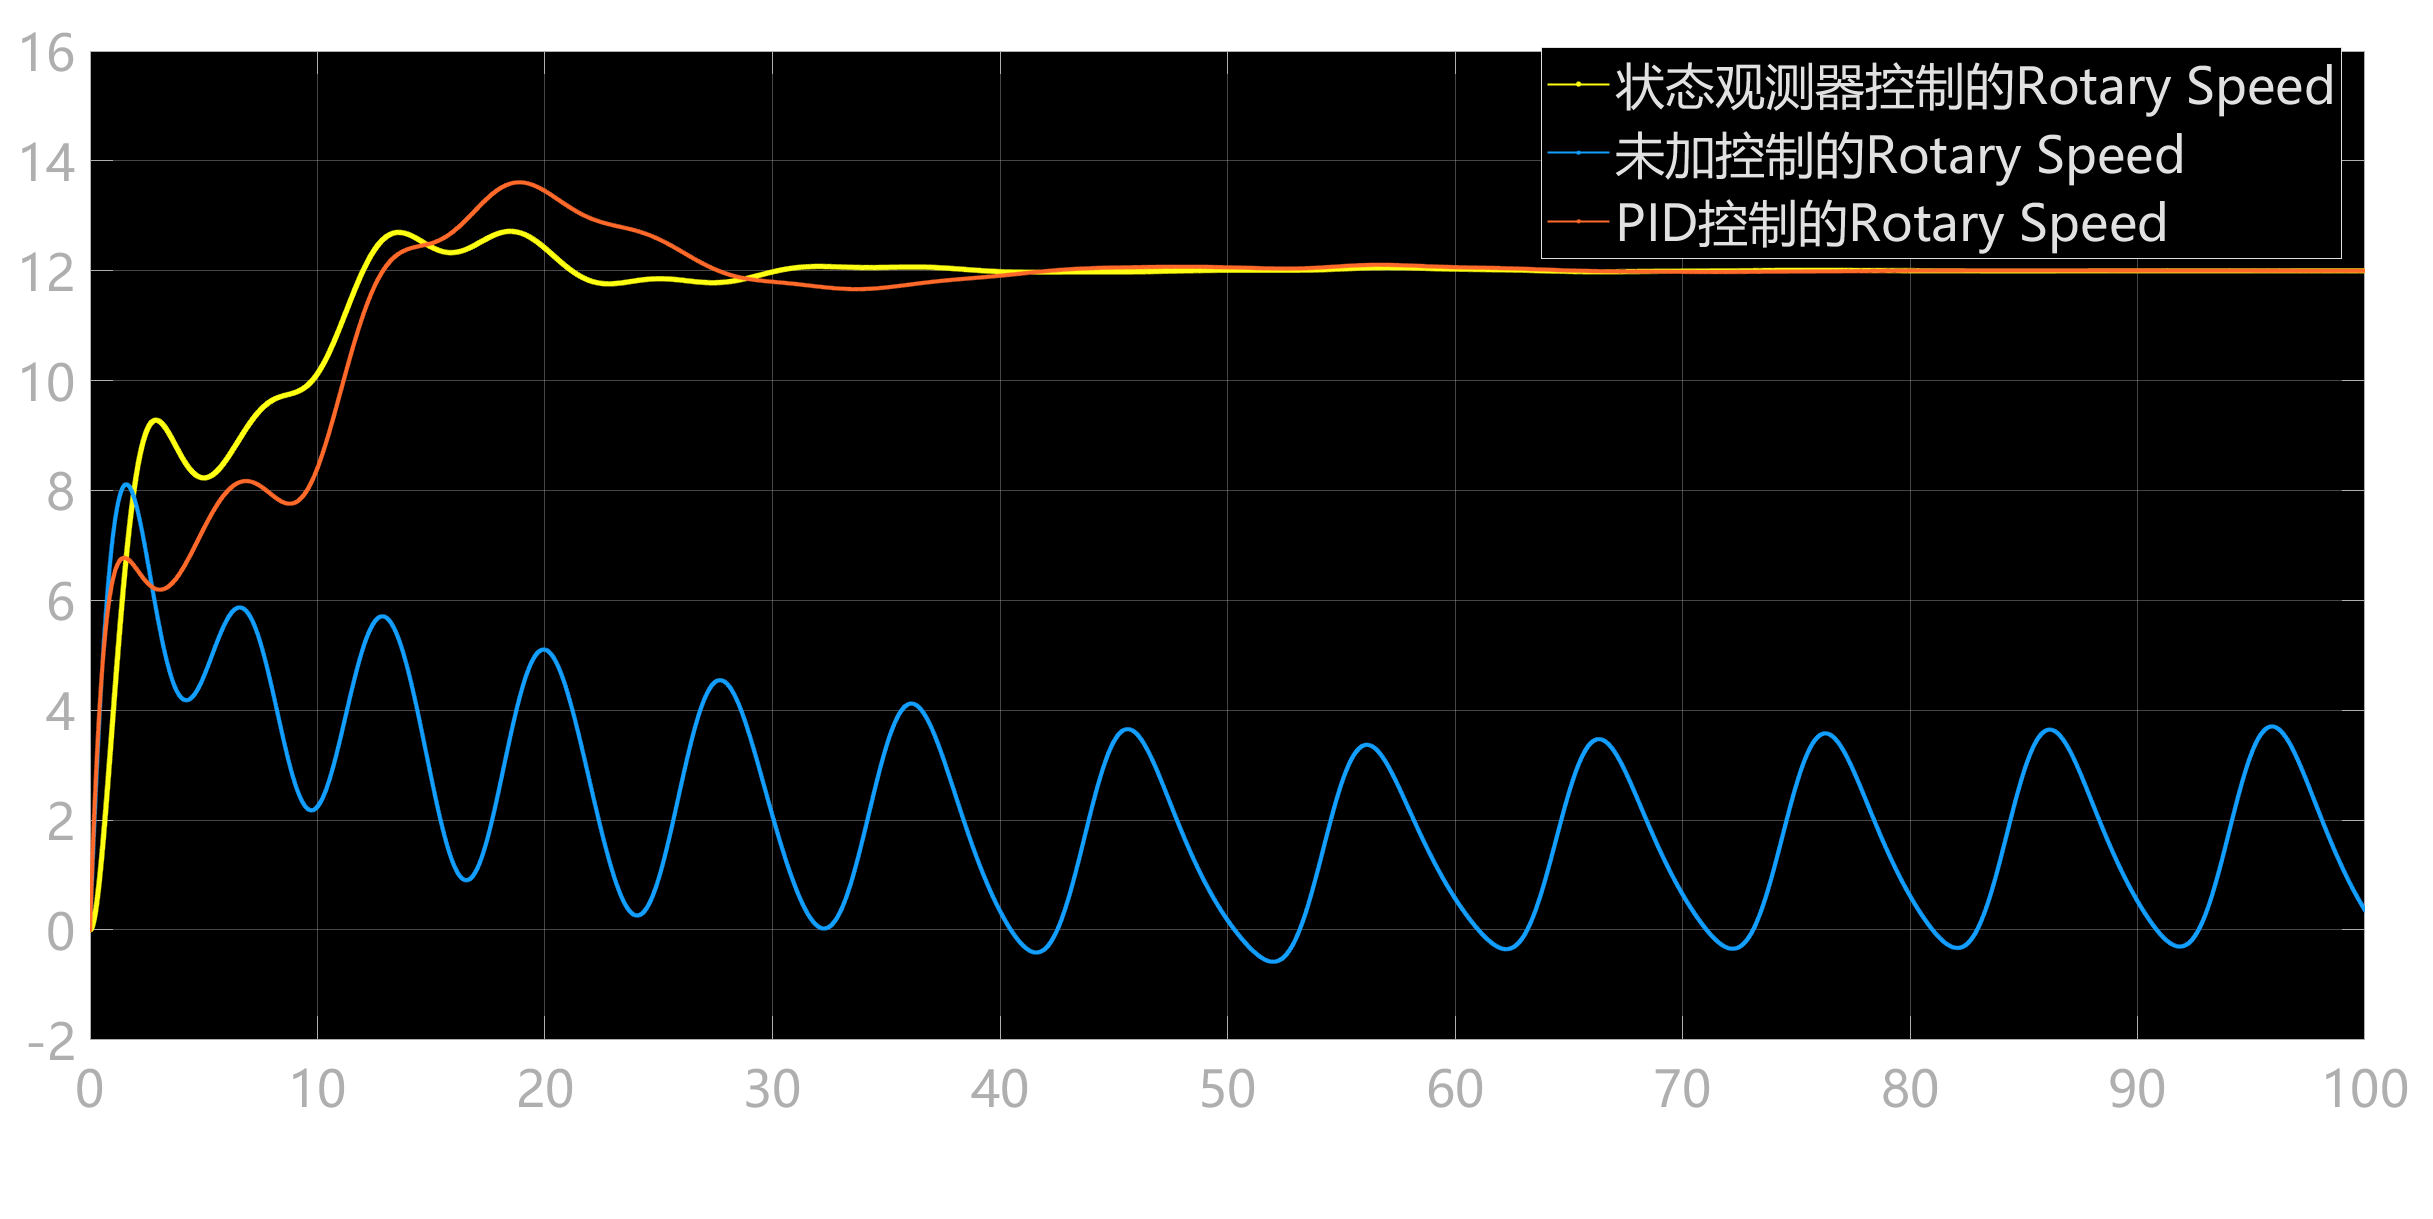
\includegraphics[width=0.45\linewidth]{fig/Rotary_Speed控制对比}
		\label{fig:compare_rotary}
	}
	\subfigure[钻头转速对比]{
		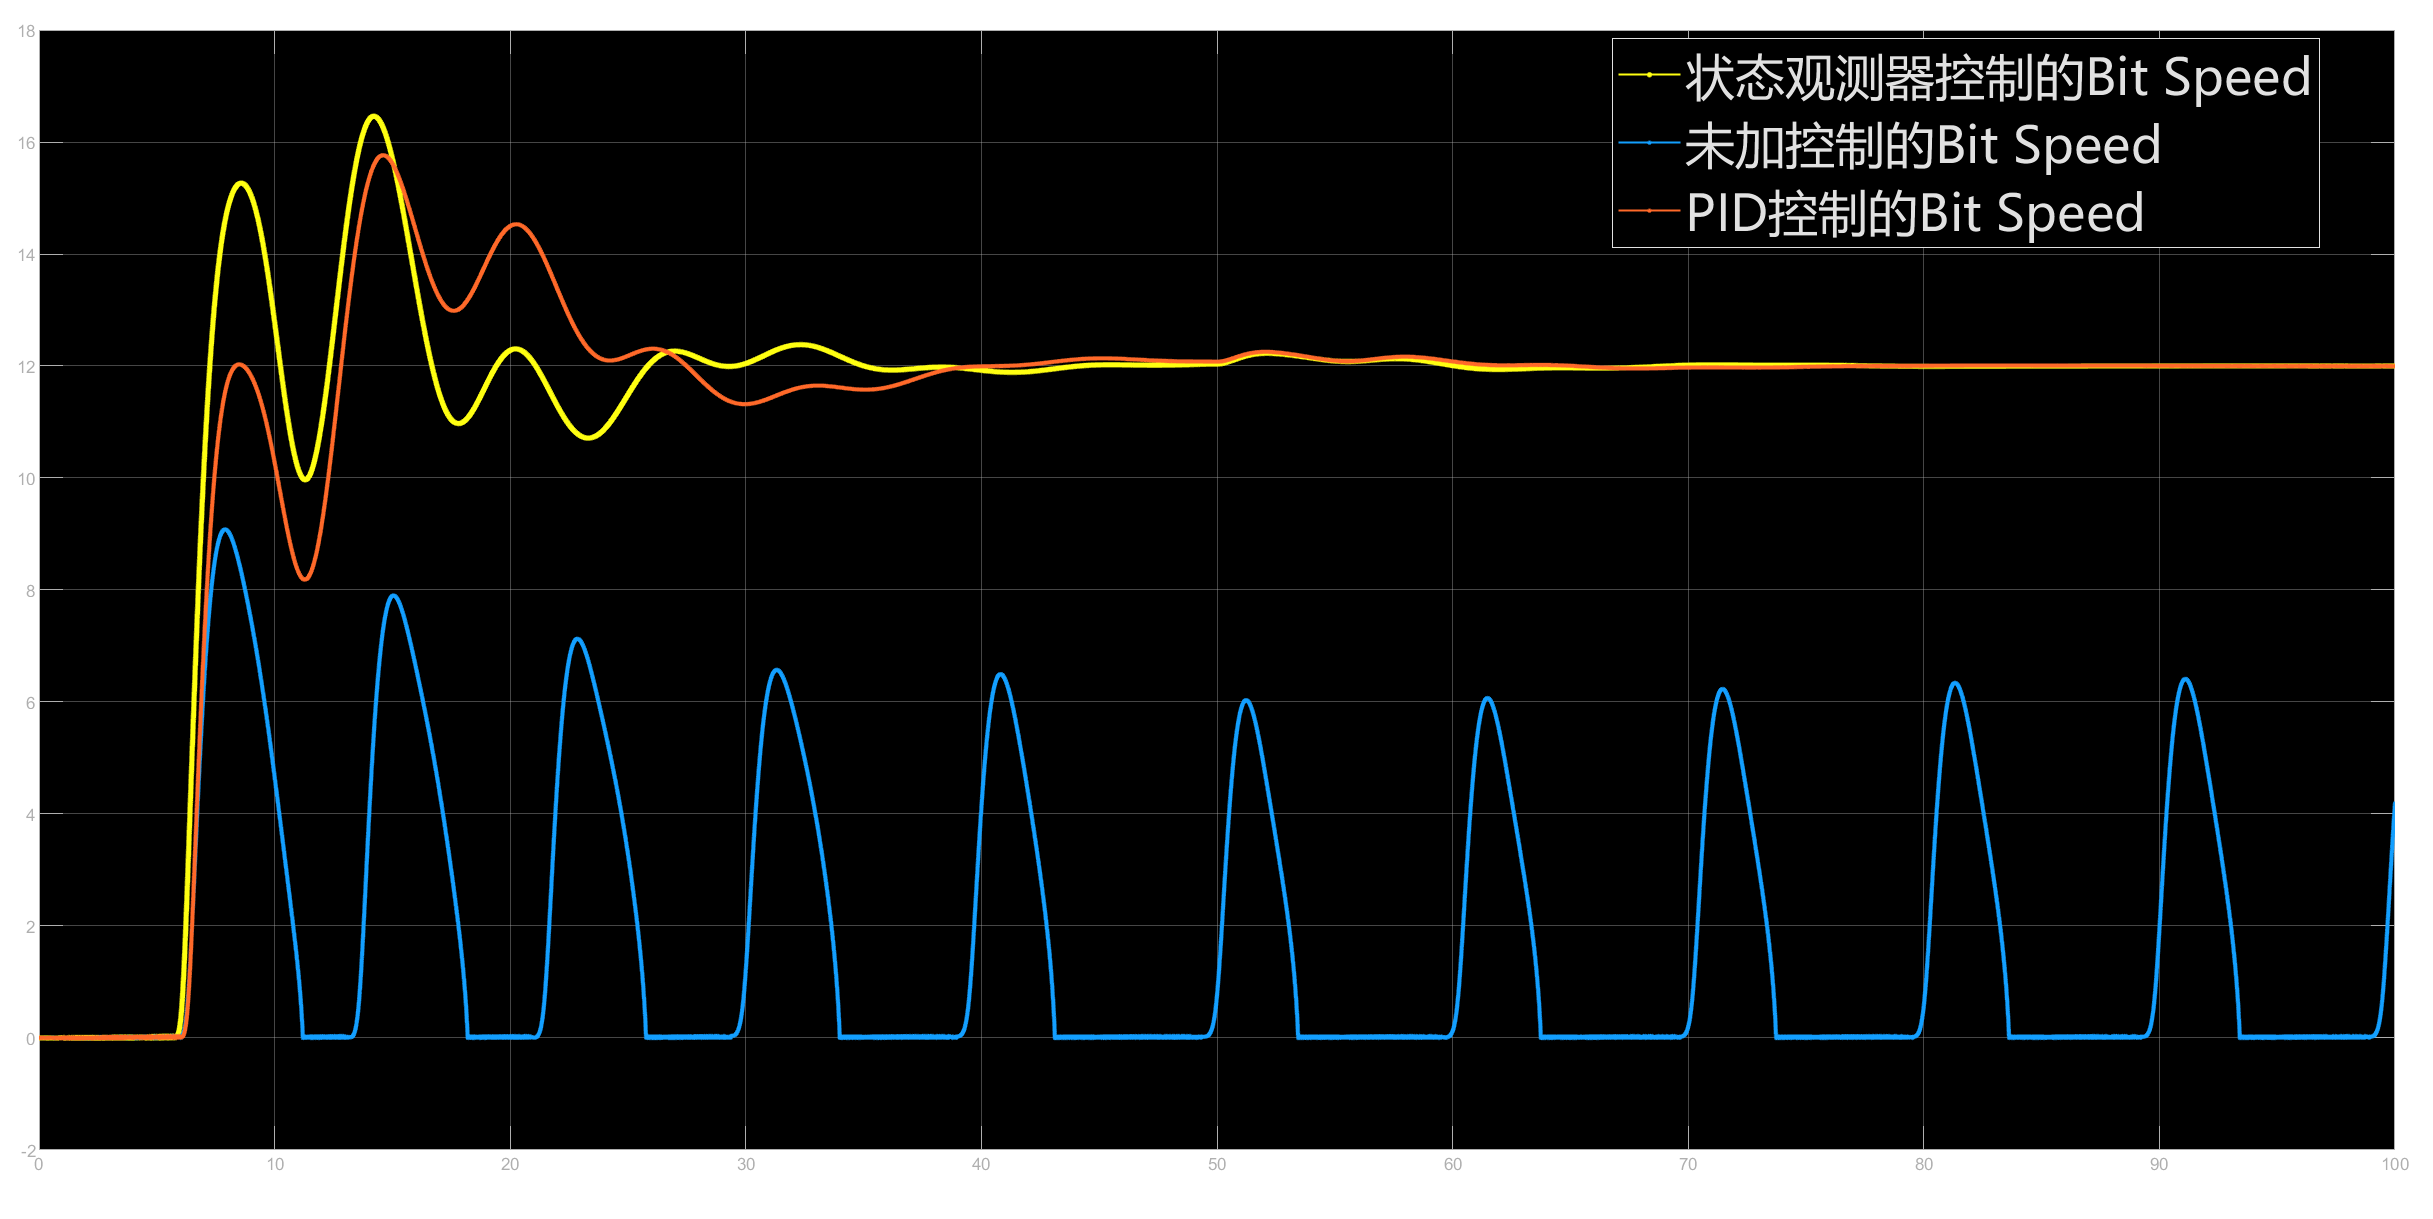
\includegraphics[width=0.45\linewidth]{fig/Bit_Speed控制对比}
		\label{fig:compare_bit}
	}
	\caption{PID控制与状态观测器控制效果的综合对比}
\end{figure}

%----------------------------------------------------------------------------------------
%	第六章 结论
%----------------------------------------------------------------------------------------
\section{结论}

本文针对深井钻柱系统的粘滑振动问题,从机理分析、建模仿真到控制策略设计进行了系统性研究。主要结论如下:
\begin{enumerate}
	\item \textbf{机理明确}:钻头与岩石界面的非线性摩擦特性(动静摩擦系数差异)是诱发粘滑振动的根源,而钻柱的长细柔性结构为振动能量的积聚与释放提供了条件。
	\item \textbf{建模有效}:构建的四自由度集总参数模型能够准确复现实际工况中的周期性粘滑现象,验证了模型的有效性。
	\item \textbf{控制优越}:相比于传统的PID控制,基于状态观测器的全状态反馈控制策略具有更优异的动态性能。它通过重构不可测的井下状态,实现了对非线性干扰的有效补偿,能够快速消除粘滑振动,保障钻头转速的平稳跟踪。
\end{enumerate}

未来的研究工作将进一步考虑钻柱轴向-扭转耦合振动的影响,并探索基于数据驱动(如深度学习)的智能控制算法在钻井工程中的应用\cite{Qiu2020}。
	
	%%----------- 参考文献 -------------------%%
	\newpage
	\bibliographystyle{gbt7714-numerical}
	\bibliography{reference}
	
\end{document}